%%%%%%%%%%%%%%%%%%%%%%%%%%%%%%%%%%%%%%%%%
% Programming/Coding Assignment
% LaTeX Template
%
% This template has been downloaded from:
% http://www.latextemplates.com
%
% Original author:
% Ted Pavlic (http://www.tedpavlic.com)
%
% Note:
% The \lipsum[#] commands throughout this template generate dummy text
% to fill the template out. These commands should all be removed when 
% writing assignment content.
%
% This template uses a Perl script as an example snippet of code, most other
% languages are also usable. Configure them in the "CODE INCLUSION 
% CONFIGURATION" section.
%
%Assignment 6
%Author Zetan
%%%%%%%%%%%%%%%%%%%%%%%%%%%%%%%%%%%%%%%%%

%----------------------------------------------------------------------------------------
%	PACKAGES AND OTHER DOCUMENT CONFIGURATIONS
%----------------------------------------------------------------------------------------

\documentclass{article}

\usepackage{fancyhdr} % Required for custom headers
\usepackage{lastpage} % Required to determine the last page for the footer
\usepackage{extramarks} % Required for headers and footers
\usepackage[usenames,dvipsnames]{color} % Required for custom colors
\usepackage{graphicx} % Required to insert images
\usepackage{listings} % Required for insertion of code
\usepackage{courier} % Required for the courier font
\usepackage{multirow}
\usepackage{listings,multicol}
\usepackage{pgfplots,pgfplotstable}
 \usepackage{amssymb}

\usepackage{url}

% Margins
\topmargin=-0.45in
\evensidemargin=0in
\oddsidemargin=0in
\textwidth=6.5in
\textheight=9.0in
\headsep=0.25in

\linespread{1.1} % Line spacing

% Set up the header and footer
\pagestyle{fancy}
\lhead{\hmwkAuthorName} % Top left header
\chead{\hmwkClass\ (\hmwkClassInstructor\ \hmwkClassTime): \hmwkTitle} % Top center head
\rhead{\firstxmark} % Top right header
\lfoot{\lastxmark} % Bottom left footer
\cfoot{} % Bottom center footer
\rfoot{Page\ \thepage\ of\ \protect\pageref{LastPage}} % Bottom right footer
\renewcommand\headrulewidth{0.4pt} % Size of the header rule
\renewcommand\footrulewidth{0.4pt} % Size of the footer rule

\setlength\parindent{0pt} % Removes all indentation from paragraphs

%----------------------------------------------------------------------------------------
%	CODE INCLUSION CONFIGURATION
%----------------------------------------------------------------------------------------
\definecolor{lightgray}{rgb}{.9,.9,.9}
\definecolor{darkgray}{rgb}{.4,.4,.4}
\definecolor{purple}{rgb}{0.65, 0.12, 0.82}
\definecolor{MyDarkGreen}{rgb}{0.0,0.4,0.0} % This is the color used for comments
\lstloadlanguages{Python} % Load python syntax for listings, for a list of other languagesftp://ftp.tex.ac.uk/tex-archive/macros/latex/contrib/listings/listings.pdf supported see: 
\lstdefinelanguage{JavaScript}{
  keywords={break, case, catch, continue, debugger, default, delete, do, else, false, finally, for, function, if, in, instanceof, new, null, return, switch, this, throw, true, try, typeof, var, void, while, with},
  morecomment=[l]{//},
  morecomment=[s]{/*}{*/},
  morestring=[b]',
  morestring=[b]",
  ndkeywords={class, export, boolean, throw, implements, import, this},
  keywordstyle=\color{blue}\bfseries,
  ndkeywordstyle=\color{darkgray}\bfseries,
  identifierstyle=\color{black},
  commentstyle=\color{purple}\ttfamily,
  stringstyle=\color{red}\ttfamily,
  sensitive=true
}
\lstset{
        frame=single, % Single frame around code
        basicstyle=\small\ttfamily, % Use small true type font
        keywordstyle=[1]\color{Blue}\bf, % python functions bold and blue
        keywordstyle=[2]\color{Purple}, % python function arguments purple
        keywordstyle=[3]\color{Blue}\underbar, % Custom functions underlined and blue
        identifierstyle=, % Nothing special about identifiers                                         
        commentstyle=\usefont{T1}{pcr}{m}{sl}\color{MyDarkGreen}\small, % Comments small dark green courier font
        stringstyle=\color{Purple}, % Strings are purple
        showstringspaces=false, % Don't put marks in string spaces
        tabsize=5, % 5 spaces per tab
        breaklines=true,
        %
        % Put standard python functions not included in the default language here
        morekeywords={rand},
        %
        % Put python function parameters here
        morekeywords=[2]{on, off, interp},
        %
        % Put user defined functions here
        morekeywords=[3]{test},
       	%
        morecomment=[l][\color{Blue}]{...}, % Line continuation (...) like blue comment
        numbers=left, % Line numbers on left
        firstnumber=1, % Line numbers start with line 1
        numberstyle=\tiny\color{Blue}, % Line numbers are blue and small
        stepnumber=5 % Line numbers go in steps of 5
}

% Creates a new command to include a pyton script, the first parameter is the filename of the script (without .py), the second parameter is the caption
\newcommand{\pythonscript}[2]{
\begin{itemize}
\item[]\lstinputlisting[language=python,caption=#2,label=#1]{#1.py}
\end{itemize}
}
% Creates a new command to include a shell script, the first parameter is the filename of the script (without .sh), the second parameter is the caption
\newcommand{\shellscript}[2]{
\begin{itemize}
\item[]\lstinputlisting[language=bash,caption=#2,label=#1]{#1.sh}
\end{itemize}
}
% Creates a new command to include a R script, the first parameter is the filename of the script (without .R), the second parameter is the caption
\newcommand{\Rscript}[2]{
\begin{itemize}
\item[]\lstinputlisting[language=R,caption=#2,label=#1]{#1.R}
\end{itemize}
}
% Creates a new command to include a java script, the first parameter is the filename of the script (without .R), the second parameter is the caption
\newcommand{\jsscript}[2]{
\begin{itemize}
\item[]\lstinputlisting[language=JavaScript,caption=#2,label=#1]{#1.js}
\end{itemize}
}
%----------------------------------------------------------------------------------------
%	DOCUMENT STRUCTURE COMMANDS
%	Skip this unless you know what you're doing
%----------------------------------------------------------------------------------------

% Header and footer for when a page split occurs within a problem environment
\newcommand{\enterProblemHeader}[1]{
\nobreak\extramarks{#1}{#1 continued on next page\ldots}\nobreak
\nobreak\extramarks{#1 (continued)}{#1 continued on next page\ldots}\nobreak
}

% Header and footer for when a page split occurs between problem environments
\newcommand{\exitProblemHeader}[1]{
\nobreak\extramarks{#1 (continued)}{#1 continued on next page\ldots}\nobreak
\nobreak\extramarks{#1}{}\nobreak
}

\setcounter{secnumdepth}{0} % Removes default section numbers
\newcounter{homeworkProblemCounter} % Creates a counter to keep track of the number of problems

\newcommand{\homeworkProblemName}{}
\newenvironment{homeworkProblem}[1][Problem \arabic{homeworkProblemCounter}]{ % Makes a new environment called homeworkProblem which takes 1 argument (custom name) but the default is "Problem #"
\stepcounter{homeworkProblemCounter} % Increase counter for number of problems
\renewcommand{\homeworkProblemName}{#1} % Assign \homeworkProblemName the name of the problem
\section{\homeworkProblemName} % Make a section in the document with the custom problem count
\enterProblemHeader{\homeworkProblemName} % Header and footer within the environment
}{
\exitProblemHeader{\homeworkProblemName} % Header and footer after the environment
}

\newcommand{\problemAnswer}[1]{ % Defines the problem answer command with the content as the only argument
\noindent\framebox[\columnwidth][c]{\begin{minipage}{0.98\columnwidth}#1\end{minipage}} % Makes the box around the problem answer and puts the content inside
}

\newcommand{\homeworkSectionName}{}
\newenvironment{homeworkSection}[1]{ % New environment for sections within homework problems, takes 1 argument - the name of the section
\renewcommand{\homeworkSectionName}{#1} % Assign \homeworkSectionName to the name of the section from the environment argument
\subsection{\homeworkSectionName} % Make a subsection with the custom name of the subsection
\enterProblemHeader{\homeworkProblemName\ [\homeworkSectionName]} % Header and footer within the environment
}{
\enterProblemHeader{\homeworkProblemName} % Header and footer after the environment
}

%----------------------------------------------------------------------------------------
%	NAME AND CLASS SECTION
%----------------------------------------------------------------------------------------

\newcommand{\hmwkTitle}{Assignment\ \#7} % Assignment title
\newcommand{\hmwkDueDate}{Thursday,\ March\ 31,\ 2016} % Due date
\newcommand{\hmwkClass}{Web Science\ cs532} % Course/class
\newcommand{\hmwkClassTime}{4:20pm} % Class/lecture time
\newcommand{\hmwkClassInstructor}{Dr.Michael.L.Nelson} % Teacher/lecturer
\newcommand{\hmwkAuthorName}{Zetan Li} % Your name

%----------------------------------------------------------------------------------------
%	TITLE PAGE
%----------------------------------------------------------------------------------------

\title{
\vspace{2in}
\textmd{\textbf{\hmwkClass:\ \hmwkTitle}}\\
\normalsize\vspace{0.1in}\small{Due\ on\ \hmwkDueDate}\\
\vspace{0.1in}\large{\textit{\hmwkClassInstructor\ \hmwkClassTime}}
\vspace{3in}
}

\author{\textbf{\hmwkAuthorName}}
\date{} % Insert date here if you want it to appear below your name

%----------------------------------------------------------------------------------------

\begin{document}

\maketitle

%----------------------------------------------------------------------------------------
%	TABLE OF CONTENTS
%----------------------------------------------------------------------------------------

%\setcounter{tocdepth}{1} % Uncomment this line if you don't want subsections listed in the ToC

\newpage
\tableofcontents
\newpage

%----------------------------------------------------------------------------------------
%	PROBLEM 1
%----------------------------------------------------------------------------------------

% To have just one problem per page, simply put a \clearpage after each problem

\begin{homeworkProblem}
Find 3 users who are closest to you in terms of age, 
gender, and occupation.  For each of those 3 users:\\
\\
- what are their top 3 favorite films?\\
- bottom 3 least favorite films?\\
\\
Based on the movie values in those 6 tables (3 users X (favorite +
least)), choose a user that you feel is most like you.  Feel 
free to note any outliers (e.g., ``I mostly identify with user 123,
except I did not like ``Ghost'' at ll").  \\
\\
This user is the ``substitute you".  \\
\centerline{SOLUTION}
To get users that are closest to me, first i have to go through all the user data and retrieve user that have the same gender, age and occupation as me.\\
Then in python, storing all the movie rating in dictionaries using user id for category. Sort the ratings and pick top 3 and bottom 3 as result.\\
\begin{figure}[h]
\centering
\caption{The users that are close to me}
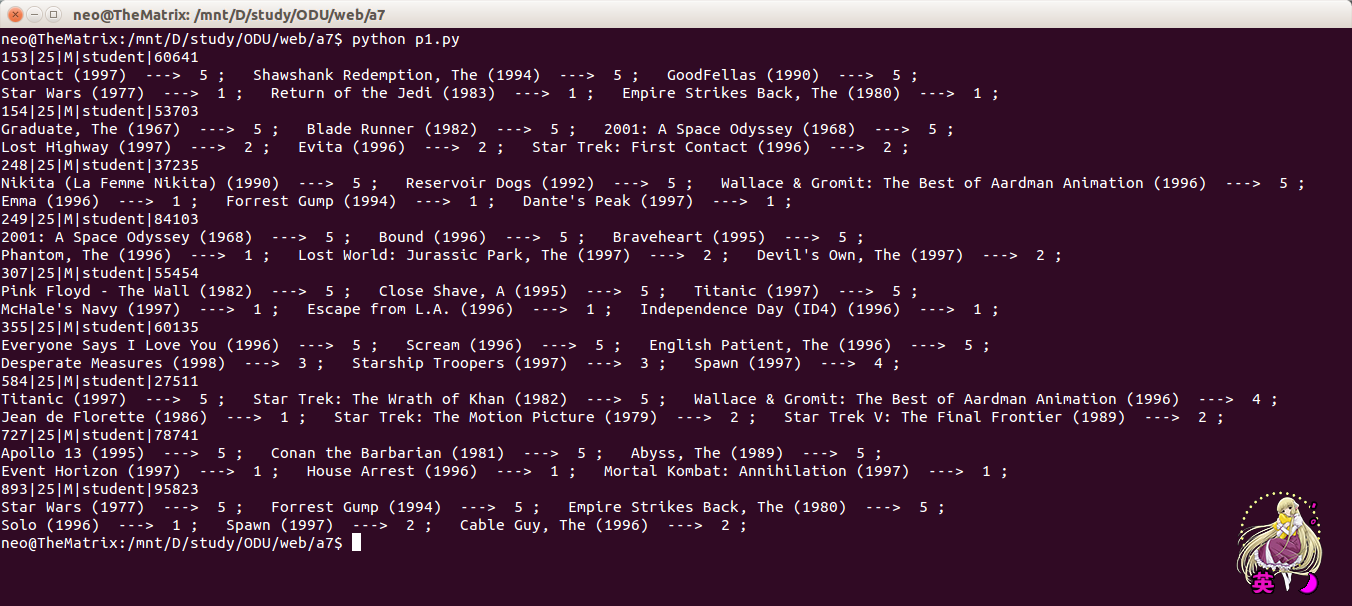
\includegraphics[scale=0.35]{users.png}
\end{figure}


Here I pick student 893 as ``substitute you", because he has Star Wars and Forrest Gump in his favorite, which is the same as me.\\

\pythonscript{p1}{Python code to get closet user and their movie preferences}
\end{homeworkProblem}
\pagebreak
%----------------------------------------------------------------------------------------
%	PROBLEM 2
%----------------------------------------------------------------------------------------
\begin{homeworkProblem}
Which 5 users are most correlated to the substitute you? Which
5 users are least correlated (i.e., negative correlation)?\\
\centerline{SOLUTION}
As in problem 1, I already stored movie ratings in the category of user ids. Next step is to explore all the users' data, pick the rating of the movie that both substitute me and them have seen, then calculate similarity.\\
Here, as I choose the pearson r for similarity, sometimes it may face ``divide by zero'' warning. In that case, distance algorithm will be performed as alternative plan.\\
When all the similarity has been calculated, give them a sort, and then we can get top 5 and bottom 5 correlated users.
\pythonscript{p2}{Python code to get correlated users}
Here's the result:\\
5 users are most correlated to the substitute you:\\
420  ( correlation: 1.0 ) \\
191  ( correlation: 1.0 ) \\
440  ( correlation: 1.0 ) \\
333  ( correlation: 1.0 ) \\
858  ( correlation: 1.0 ) \\
5 users are least correlated to the substitute you:\\
604 ( correlation: -1.0 ) \\
309 ( correlation: -1.0 ) \\
212 ( correlation: -1.0 ) \\
469 ( correlation: -1.0 ) \\
319 ( correlation: -1.0 ) \\
\end{homeworkProblem}
\pagebreak
%----------------------------------------------------------------------------------------
%	PROBLEM 3
%----------------------------------------------------------------------------------------
\begin{homeworkProblem}
Compute ratings for all the films that the substitute you
hasn't seen.  Provide a list of the top 5 recommendations for films
that the substitute you should see.  Provide a list of the bottom
5 recommendations (i.e., films the substitute you is almost certain
to hate).\\
\centerline{SOLUTION}
To get most likely rating for the film that one hasn't seen, we have to calculate the weighted average rating of all other users.\\
Note that here we ignored the user that have zero and negative similarity. (If those data are included, the result will be weird, with average rating that more than 5)\\
Sorting the weighted average rating of all the film that substitute me haven't seen, and pick top 5 and bottom 5 as result.
\pythonscript{p3}{Python code to get estimated rating of unseen movies}
The result is:\\
Top 5 recommendations for films\\
Entertaining Angels: The Dorothy Day Story (1996)  |    Most likely rating:  5.0\\
Great Day in Harlem, A (1994)  |    Most likely rating:  5.0\\
They Made Me a Criminal (1939)   |   Most likely rating:  5.0\\
Someone Else's America (1995)   |   Most likely rating:  5.0\\
Saint of Fort Washington, The (1993)   |   Most likely rating:  5.0\\
\\
Bottom 5 recommendations for films\\
Event Horizon (1997)  |    Most likely rating:  0\\
Mimic (1997)  |    Most likely rating:  0\\
Rock, The (1996)  |    Most likely rating:  0\\
Twister (1996)  |    Most likely rating:  0\\
Circle of Friends (1995)  |    Most likely rating:  0\\
\end{homeworkProblem}
\pagebreak
%----------------------------------------------------------------------------------------
%	PROBLEM 4
%----------------------------------------------------------------------------------------
\begin{homeworkProblem}
Choose your (the real you, not the substitute you) favorite and
least favorite film from the data.  For each film, generate a list
of the top 5 most correlated and bottom 5 least correlated films.
Based on your knowledge of the resulting films, do you agree with
the results?  In other words, do you personally like / dislike
the resulting films?\\
\centerline{SOLUTION}
Exploring all the films in the file, I choose the film below as my input data:\\
Favorite movie:\\
121|Independence Day (ID4) (1996)\\
\\
Least favorate movie:\\
870|Touch (1997)\\
\\
To get recommendations on movies instead of users, we switch the row and column and calculate similarity of the movies as we did with users.\\
This time, we store the user rating in the category of movie id instead of user id.\\
Then pick the top 5 and bottom 5 movie from movie table that sorted by similarity.\\
\pythonscript{p4}{Python code to calculate similarity of the given movie}
The result is:\\
\\
Favorate movie: 121|Independence Day (ID4) (1996)\\
Top 5 most correlated movies:\\
Wife, The (1995)  ( correlation: 1.0 ) \\
Savage Nights (Nuits fauves, Les) (1992)  ( correlation: 1.0 ) \\
Collectionneuse, La (1967)  ( correlation: 1.0 ) \\
Truth or Consequences, N.M. (1997)  ( correlation: 1.0 ) \\
Intimate Relations (1996)  ( correlation: 1.0 ) \\
\\
Bottom 5 least correlated movies:\\
Crows and Sparrows (1949) ( correlation: -1.0 ) \\
Kicked in the Head (1997) ( correlation: -1.0 ) \\
Underworld (1997) ( correlation: -1.0 ) \\
Johnny 100 Pesos (1993) ( correlation: -1.0 ) \\
Forbidden Christ, The (Cristo proibito, Il) (1950) ( correlation: -1.0 ) \\
\\
=======================================
\\
Least favorate movie: 870|Touch (1997)\\
Top 5 most correlated movies:\\
Hoodlum (1997)  ( correlation: 1.0 ) \\
Ulee's Gold (1997)  ( correlation: 1.0 ) \\
Rosewood (1997)  ( correlation: 1.0 ) \\
Good Will Hunting (1997)  ( correlation: 1.0 ) \\
Restoration (1995)  ( correlation: 1.0 ) \\
\\
Bottom 5 least correlated movies:\\
I Know What You Did Last Summer (1997) ( correlation: -1.0 ) \\
Smilla's Sense of Snow (1997) ( correlation: -1.0 ) \\
Halloween: The Curse of Michael Myers (1995) ( correlation: -1.0 ) \\
Amistad (1997) ( correlation: -1.0 ) \\
She's So Lovely (1997) ( correlation: -1.0 ) \\
\\
For me this result seems a little weird to me. I don't know the movie listed above, and when i try to get some information about them though google, some of them seems interesting but in totally different category.
\end{homeworkProblem}
%\bibliographystyle{plain}
%\bibliography{ref}
\end{document}